\documentclass[a1papper, portrait]{tikzposter}
\usepackage[utf8]{inputenc}

\usepackage{url}
\usepackage{indentfirst}

\usepackage{algorithmic}
\usepackage{algorithm}

% изменение размера шрифта > больше чем максимальный
\makeatletter
\input{theguy30pt.clo}
\makeatother

\title{Deep: optimizer with embedded interpreter}
\author{A.~V.~Svichkarev, K.~N.~Kozlov}
\institute{System biology and bioinformatics lab, IAMM,\\
    Peter the Great St.Petersburg Polytechnic University,
    St.Petersburg, Russia\\[0.5cm]
    email: \url{tolik0393@bionet.nsc.ru}
}

\usetheme{Envelope}

\begin{document}

\maketitle

\begin{columns}
    \column{0.4}
    \block{1. Introduction}{
        Problem of parameter estimation
        for systems biology is challenging due:
        \begin{itemize}
            \item[-] diversity of biomedical applications,
            \item[-] large heterogeneous datasets,
            \item[-] computationally expensive calculations
                using interpreted languages.
        \end{itemize}
        (P.~Mendes and D.~Kell, 1998)
    }

    \column{0.6}
    \block{2. Differential Evolution\\Entirely Parallel method}{
        \begin{algorithm}[H]
            \begin{algorithmic}
                \STATE{INITIALIZATION:} The population is initialized randomly.
                \STATE{Iteration = 0}
                \WHILE{Stopping criterion is not met}
                \STATE{Iteration = Iteration + 1}
                \STATE{RECOMBINATION:}
                \IF{The predefined number of iterations $\Xi$ passed.}
                \STATE{Make Scatter Search Step}
                \ELSE
                \FORALL{individuals in population}
                \STATE{{\bf recombine} (individual)}
                \ENDFOR
                \ENDIF
                \STATE{EVALUATION:}
                \STATE{{\bf objfunc} (population)}
                \STATE{SELECTION:}
                \FORALL{offsprings}
                \STATE{{\bf select} (offspring)}
                \ENDFOR
                \STATE{ADAPTATION:}
                \STATE{Update scaling and crossover parameters.}
                \IF{The predefined number of iterations $\Theta$ passed.}
                \STATE{Substitute $\Psi$ oldest individuals with the best ones.}
                \ENDIF
                \STATE{Sort the population members by age and by quality.}
                \ENDWHILE
            \end{algorithmic}
        \end{algorithm}

        (K.~Kozlov and A.~Samsonov, 2011).
    }
\end{columns}

\begin{columns}
    \column{0.45}
    \block{3. Our approach}{
        Reduces the
        communication bottleneck
        between DEEP and objective function:
        \begin{itemize}
            \item[-] Master-slave architecture,
            \item[-] The pool of embedded identical interpreters-slaves,
            \item[-] Asynchronous queue of tasks-master.
        \end{itemize}
    }
    \block{Tukey test\\of computation time}
    {
        \begin{tikzfigure}
            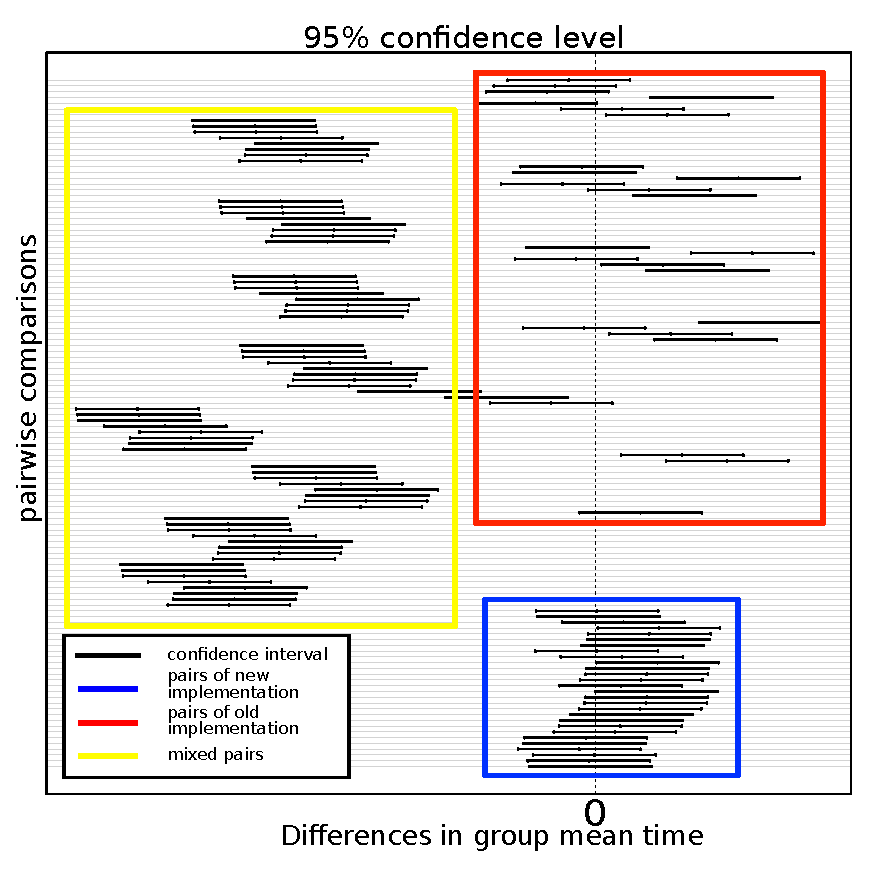
\includegraphics[width=0.4\textwidth]{images/tukey_eng}
        \end{tikzfigure}
    }
    \block{4. Discussion}{
        \begin{enumerate}
            \item Statistical significant speed up,
            \item No significant increase RAM,
            \item Different interpreted languages R, Octave, Python, etc.
        \end{enumerate}
    }
    \block{Availability}{
        DEEP: \url{http://deepmethod.sf.net}
    }
    \column{0.55}
    \block{EGFR endocytosis in HeLa cells}
    {
        The trajectory segmentation by fitting parameters of HMM with two states:
        \begin{itemize}
            \item[-] \textit{diffusion:} \textbf{black segments}
            \item[-] \textit{directional motion:} {\color{green}\textbf{green segments}}
        \end{itemize}
        \begin{tikzfigure}
            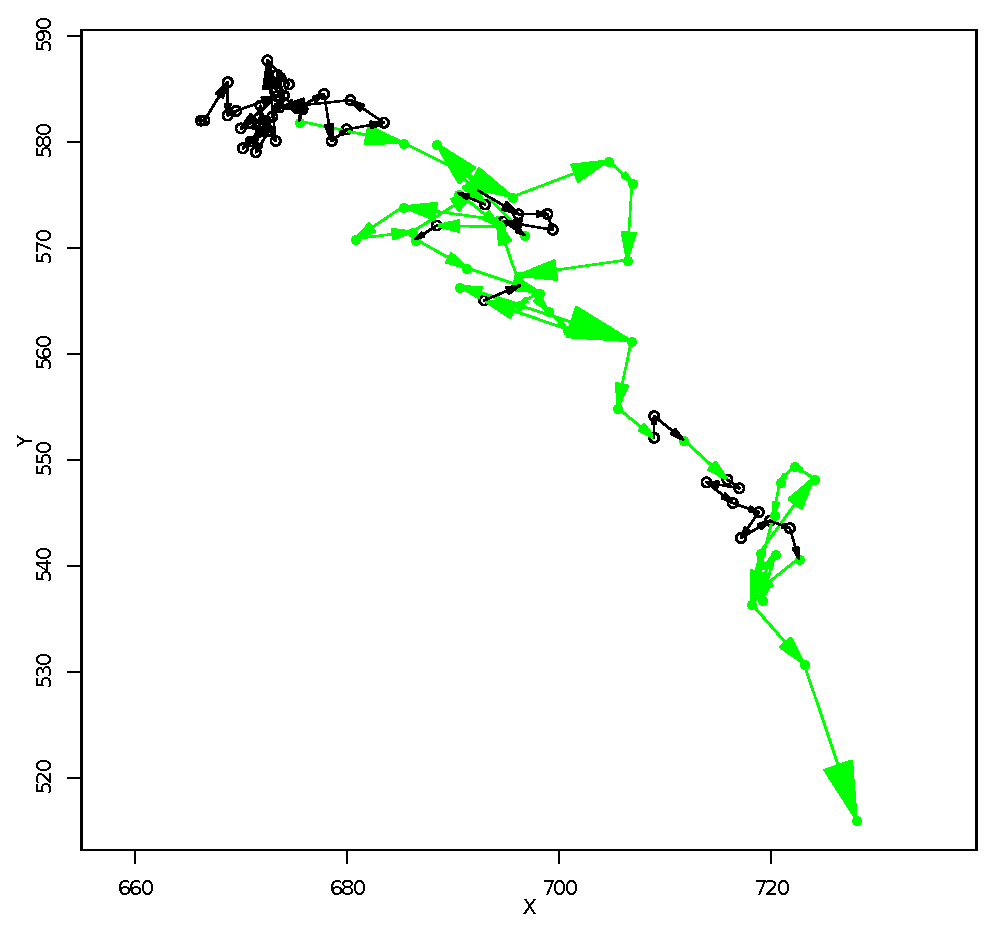
\includegraphics[width=0.3\textwidth]{images/track2}
        \end{tikzfigure}
    }
    \block{Comparison of performance}
    {
        \begin{tikzfigure}
            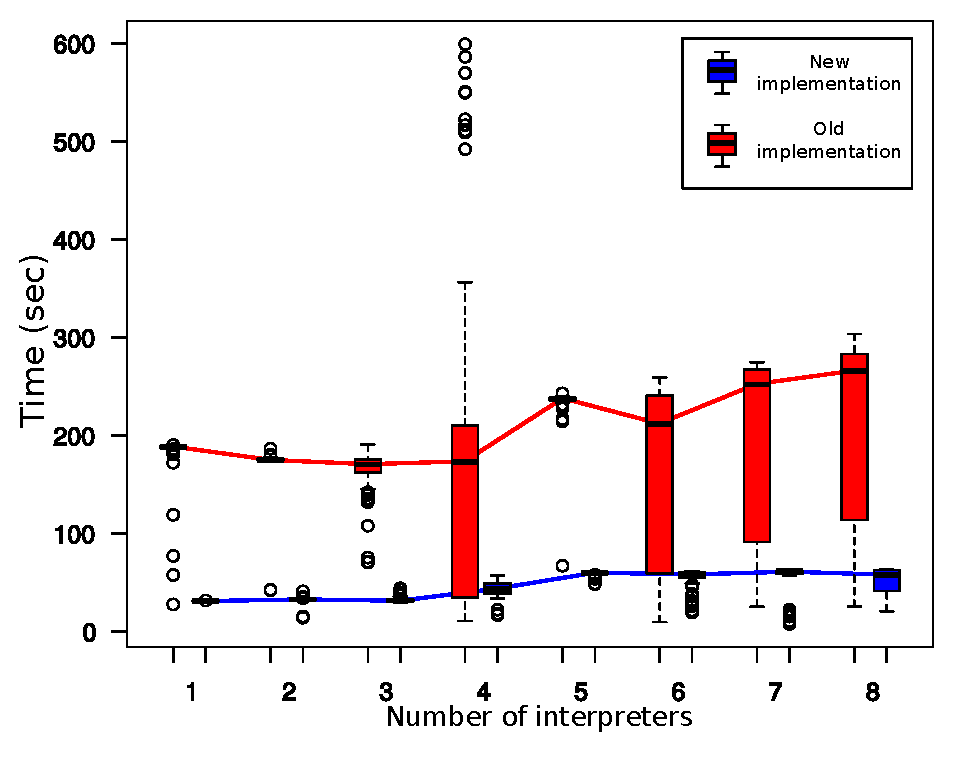
\includegraphics[width=0.45\textwidth]{images/m5_eng}
        \end{tikzfigure}
        \centering
        The new method outperformed
        the original one by the
        factor of 4
        in case of using 4
        parallel threads and 4
        interpreters.
    }
\end{columns}

\end{document}
